\documentclass[a4paper, border=3.14mm]{article}

\usepackage{xcolor}
\usepackage{tikz}
\usepackage{worldflags}

\begin{document}

\definecolor{roc-blue}{cmyk}{1.0, 0.8, 0, 0.2} %C100-M80-Y0-K20
\definecolor{roc-red}{cmyk}{0, 1, 1, 0.05} % C0-M100-Y100-K5~10


\begin{tikzpicture}
    % % Draw the red background
    % \fill[roc-red] (0,0) rectangle (12,8);
    
    % % Draw the blue rectangle
    % \fill[roc-blue] (0,4) rectangle (6,8);

    % % Draw the white sun
    % \filldraw[white] (3,6) circle (1.0);

    % % Draw the sun rays
    % \foreach \angle in {0,30,...,330} {
    %     \filldraw[white] (3,6) -- ++(\angle:1.5) -- ++(\angle+15:0.75) -- cycle;
    % }

\node {Republic of China:};
    \worldflag[width=2cm]{NATO} \\
    % \worldflag[width=2cm]{TW} \\

\node {People's Republic of China:};
    \worldflag[width=2cm]{CN} \\

\node {United States of American:};
    \worldflag[width=2cm]{USA} \\

\node {United Kindom};
    \worldflag[width=2cm]{UK} \\

\node {France:};
    \worldflag[width=2cm]{FR} \\

\end{tikzpicture}

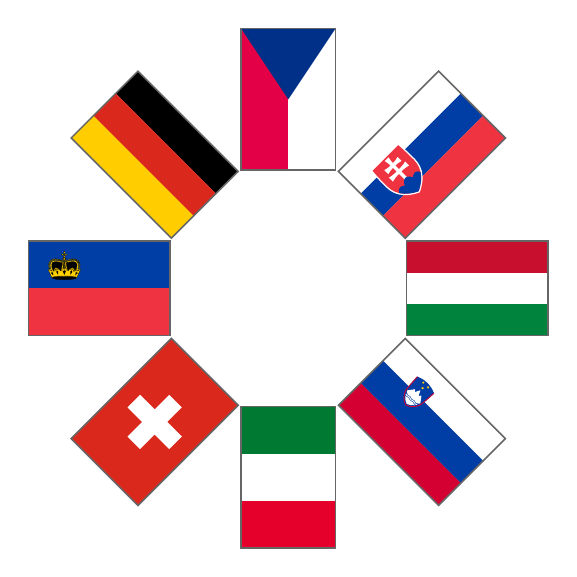
\begin{tikzpicture}
\flagsdefault[width=12mm,length=18mm]

\foreach \c/\n in {HU/0,SK/1,IT/6,SI/7}
    \pic [country=\c,rotate=\n*45]
        at (\n*45:24mm) {worldflag};

\foreach \c/\n in {CZ/2,DE/3,LI/4,CH/5}
    \pic [country=\c,rotate=\n*45-180]
        at (\n*45:24mm) {worldflag};
\end{tikzpicture}

\end{document}


